  \documentclass[final]{beamer} % beamer 3.10: do NOT use option hyperref={pdfpagelabels=false} !
%\documentclass[final,hyperref={pdfpagelabels=false}]{beamer} % beamer 3.07: get rid of beamer warnings
\mode<presentation> {  %% check http://www-i6.informatik.rwth-aachen.de/~dreuw/latexbeamerposter.php for examples
	\usetheme{Berlin}    %% you should define your own theme e.g. for big headlines using your own logos 
}
\setbeamertemplate{caption}[numbered]

\usepackage[english]{babel}
\usepackage[latin1]{inputenc}
\usepackage{amsmath,amsthm, amssymb, latexsym}
%\usepackage{times}\usefonttheme{professionalfonts}  % times is obsolete
\usefonttheme[onlymath]{serif}
\boldmath
\usepackage[orientation=landscape,size=a1,debug]{beamerposter}
\usepackage{float}    
\usepackage{subcaption}              % e.g. for DIN-A0 poster
%\usepackage[orientation=portrait,size=a1,scale=1.4,grid,debug]{beamerposter}                  % e.g. for DIN-A1 poster, with optional grid and debug output
%\usepackage[size=custom,width=200,height=120,scale=2,debug]{beamerposter}                     % e.g. for custom size poster
%\usepackage[orientation=portrait,size=a0,scale=1.0,printer=rwth-glossy-uv.df]{beamerposter}   % e.g. for DIN-A0 poster with rwth-glossy-uv printer check
% ...
%
\title[Fancy Posters]{Prometheus AI}
\author{Sean Stappas}
\institute[RWTH Aachen University]{McGill University}
\date{Jul. 31th, 2007}

% edit this depending on how tall your header is. We should make this scaling automatic :-/
\newlength{\columnheight}
\setlength{\columnheight}{104cm}


\begin{document}
\begin{columns}
	\begin{column}{.3\textwidth}
			\begin{block}{Introduction}
			\end{block}
			\begin{block}{Background}
				\begin{figure}[!htb]
					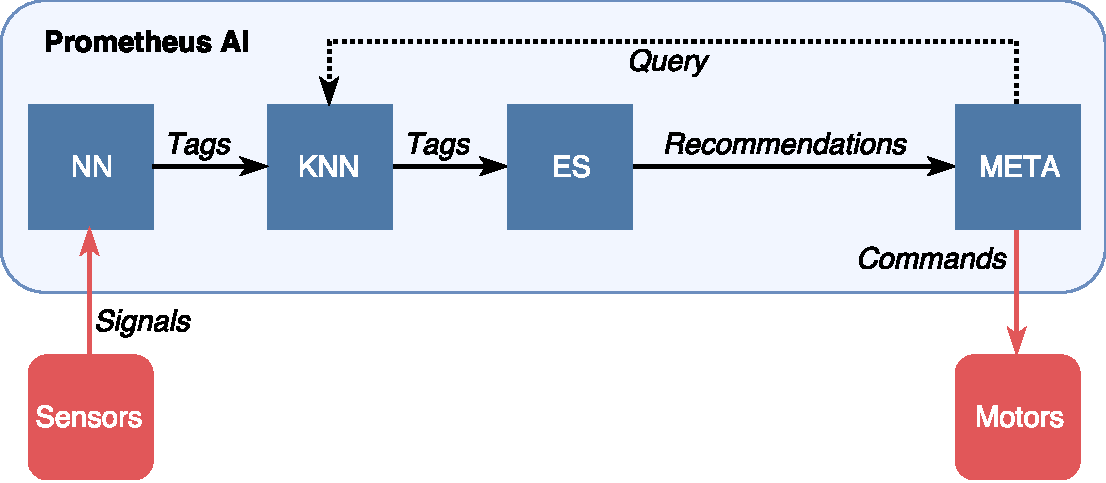
\includegraphics[width=\textwidth]{figures/ai_model_labeled.pdf}
					\caption{Prometheus AI model with labeled input and output.}
					\label{model_labeled}
				\end{figure}
			
				\begin{figure}[!htb]
					\centering
					\caption{Thinking forwards in the KNN.}
				\end{figure}
				\begin{figure}[!htb]
					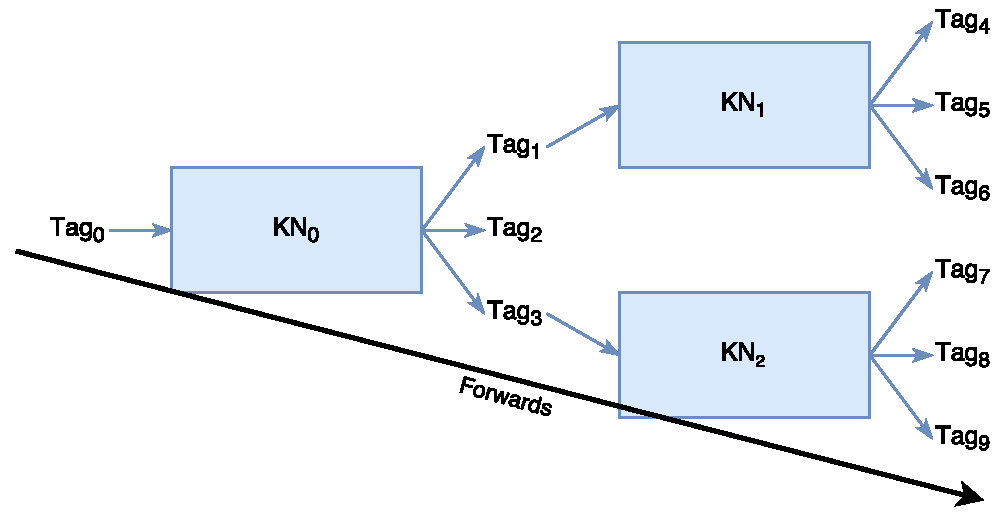
\includegraphics[width=0.5\columnwidth]{figures/forwards_thinking.pdf}
					\caption{Thinking forwards in the KNN.}
					\label{think_forwards}
				\end{figure}
				
				\begin{figure}[!htb]
					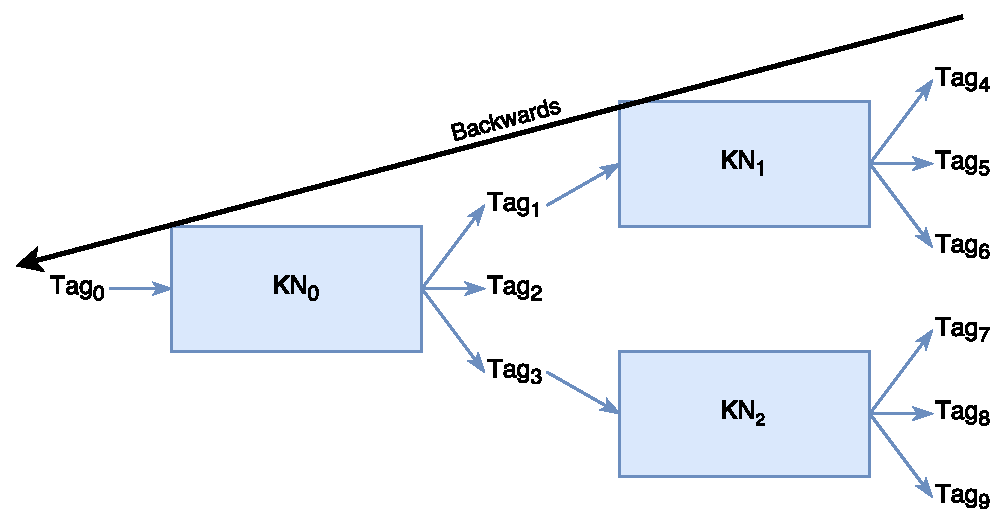
\includegraphics[width=0.5\columnwidth]{figures/backwards_thinking.pdf}
					\caption{Thinking backwards in the KNN.}
					\label{think_backwards}
				\end{figure}
				
				\begin{figure}[!htb]
					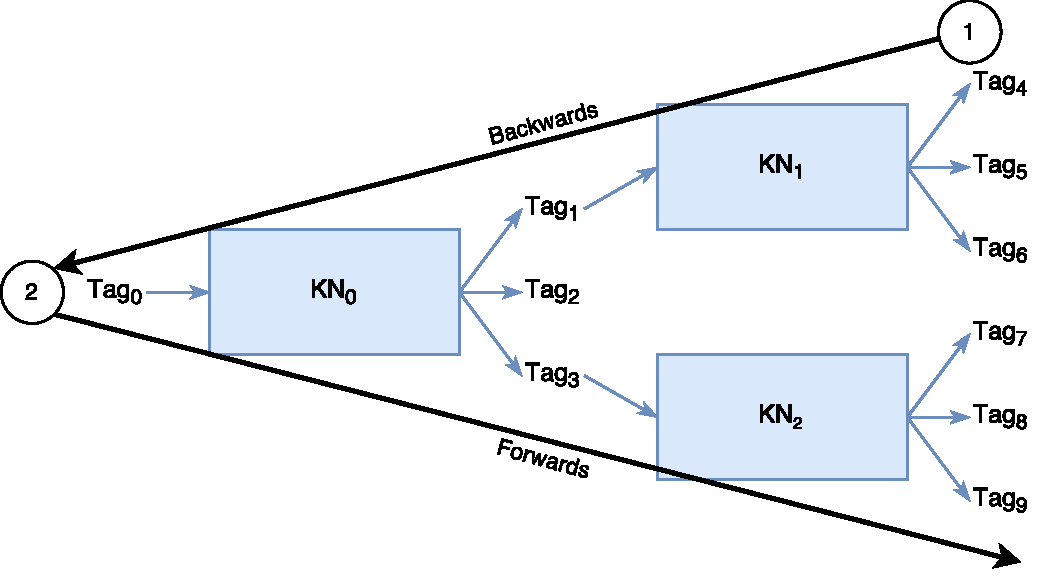
\includegraphics[width=0.5\columnwidth]{figures/lambda_thinking.pdf}
					\caption{Lambda thinking in the KNN.}
					\label{think_lambda}
				\end{figure}
			\end{block}
			\begin{block}{Problem}
			\end{block}
	\end{column}
	\begin{column}{.35\textwidth}
		\begin{block}{Design}
		\end{block}
		\begin{block}{Implementation}
		\begin{figure}[!htb]
			\centering
			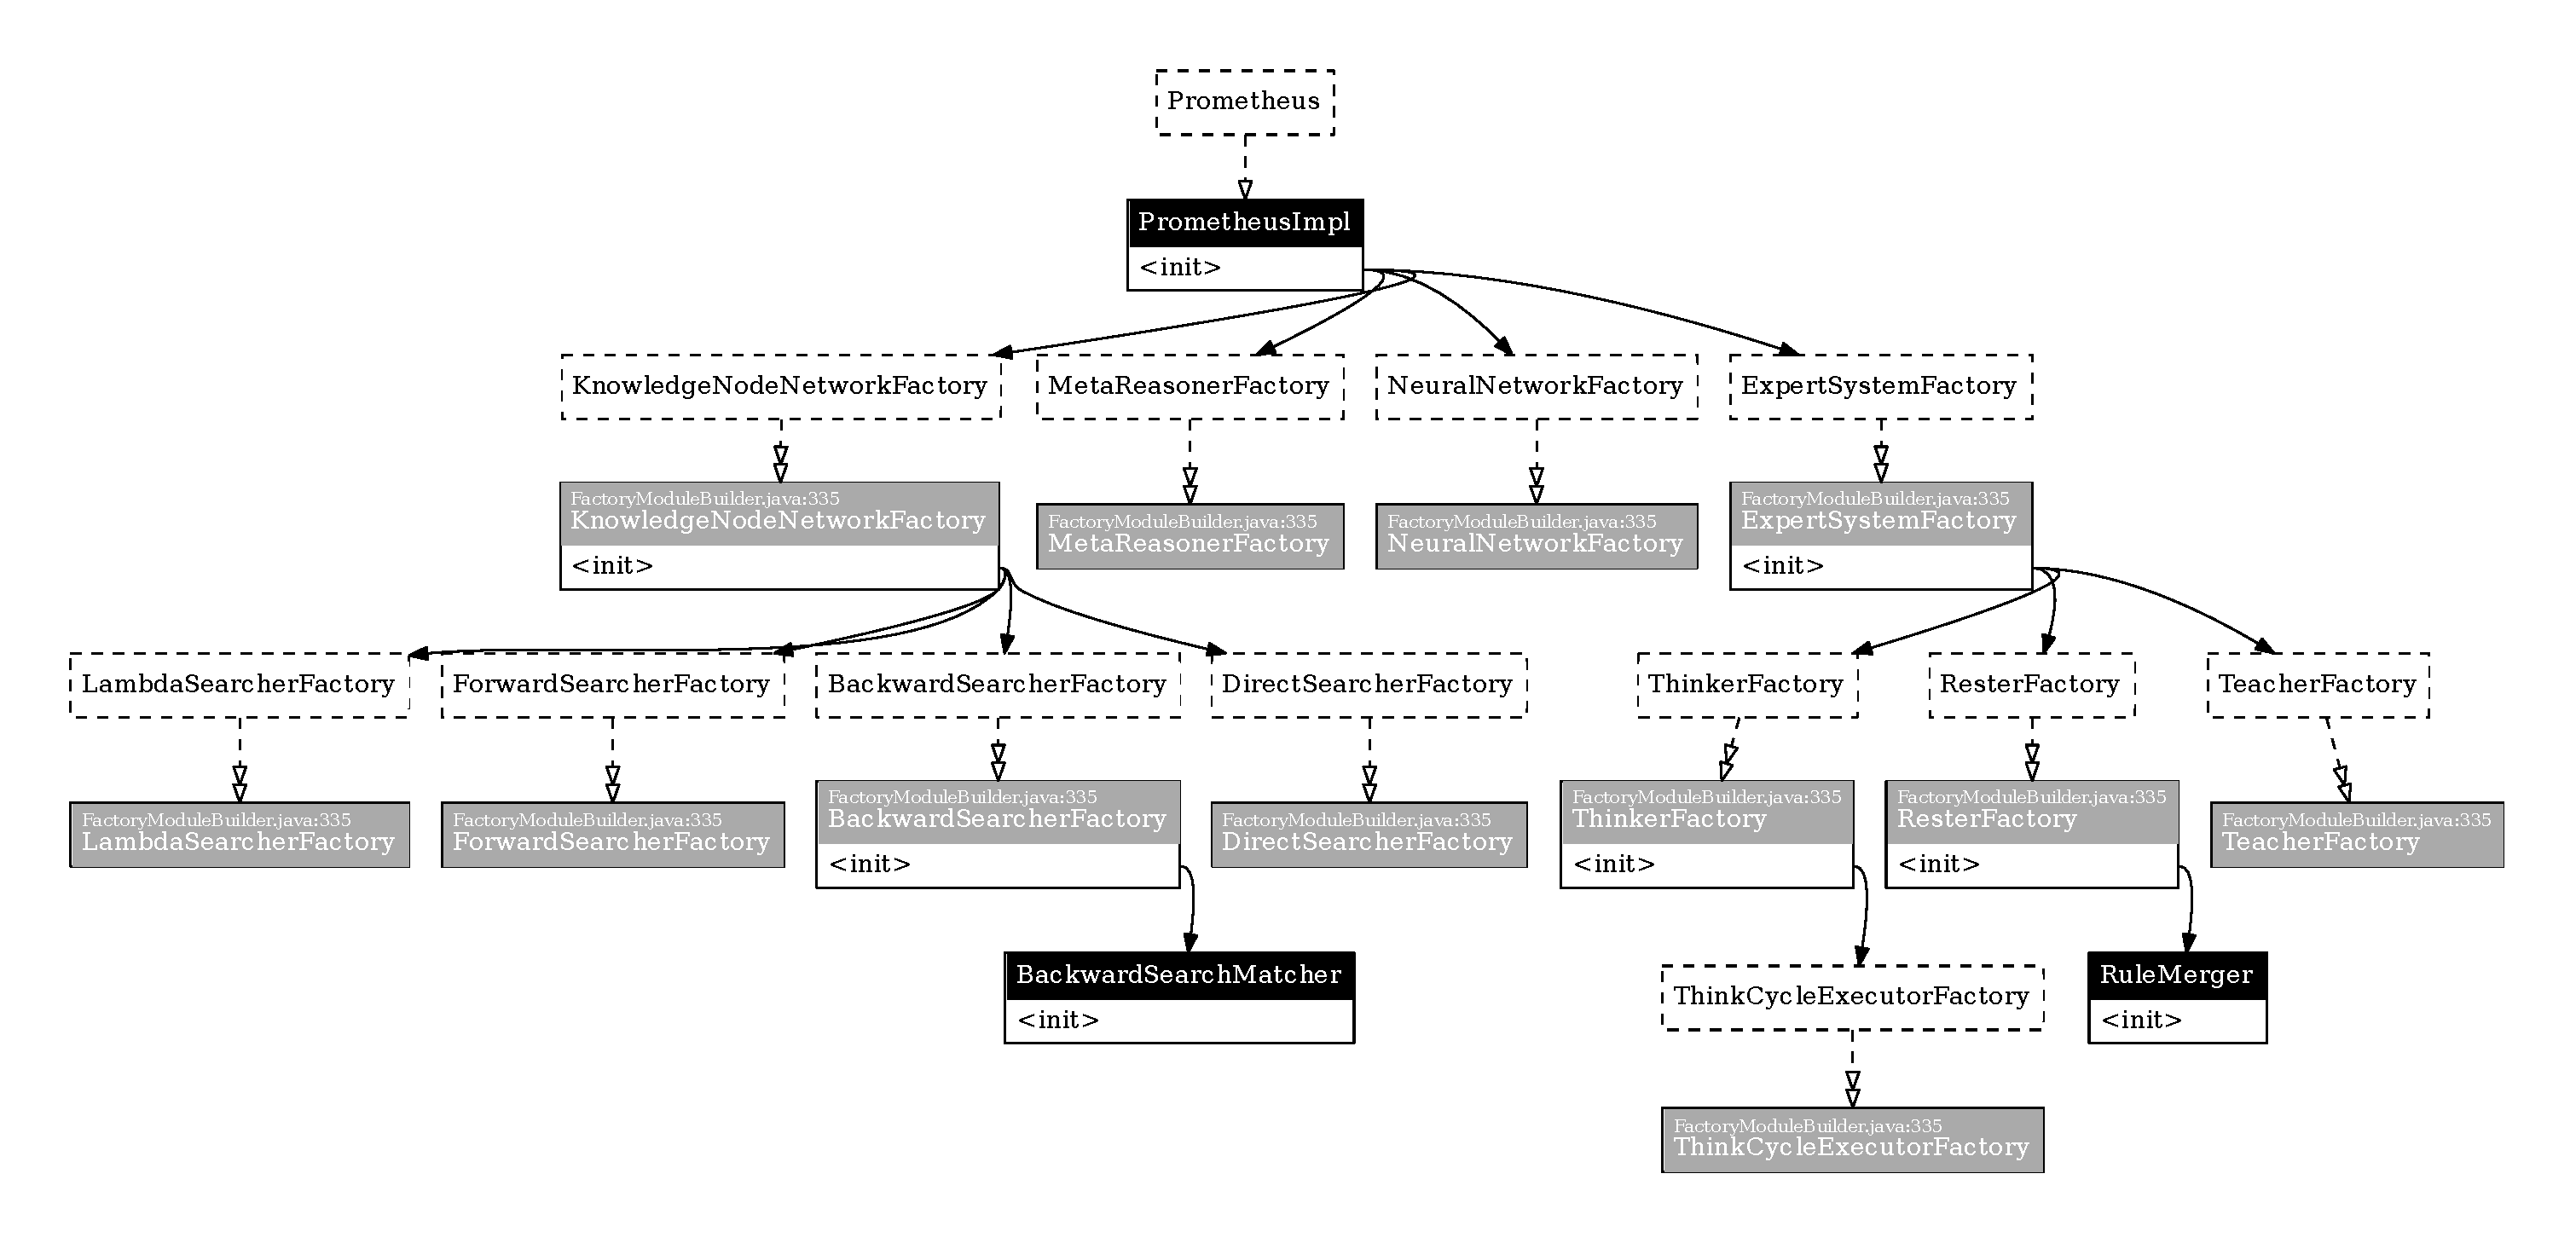
\includegraphics[width=\columnwidth]{figures/guice_graph.pdf}
			\caption
			{Guice dependency graph.}
		\end{figure}
	
		\begin{figure}[!htb]
			\centering
			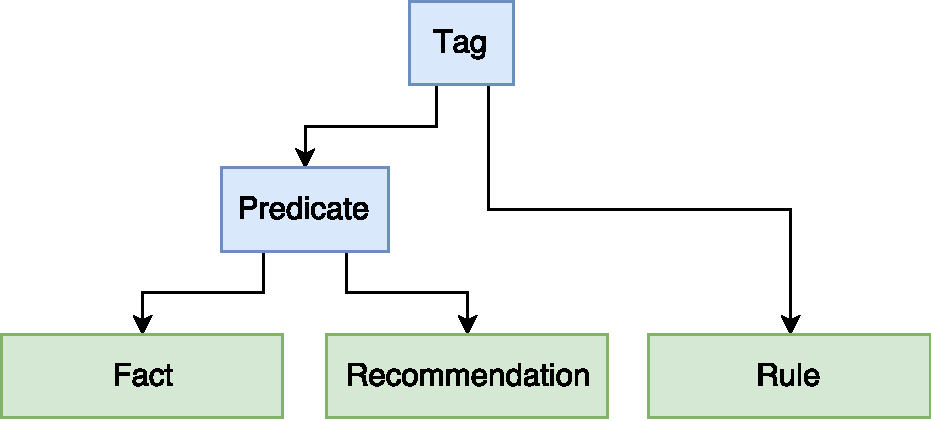
\includegraphics[width=0.5\columnwidth]{figures/prometheus_tags.pdf}
			\caption
			{Tag inheritance graph.}
		\end{figure}
		
		\begin{figure}[!htb]
			\centering
%			\begin{subfigure}[!htb]{0.3\textwidth}
%				\centering
%				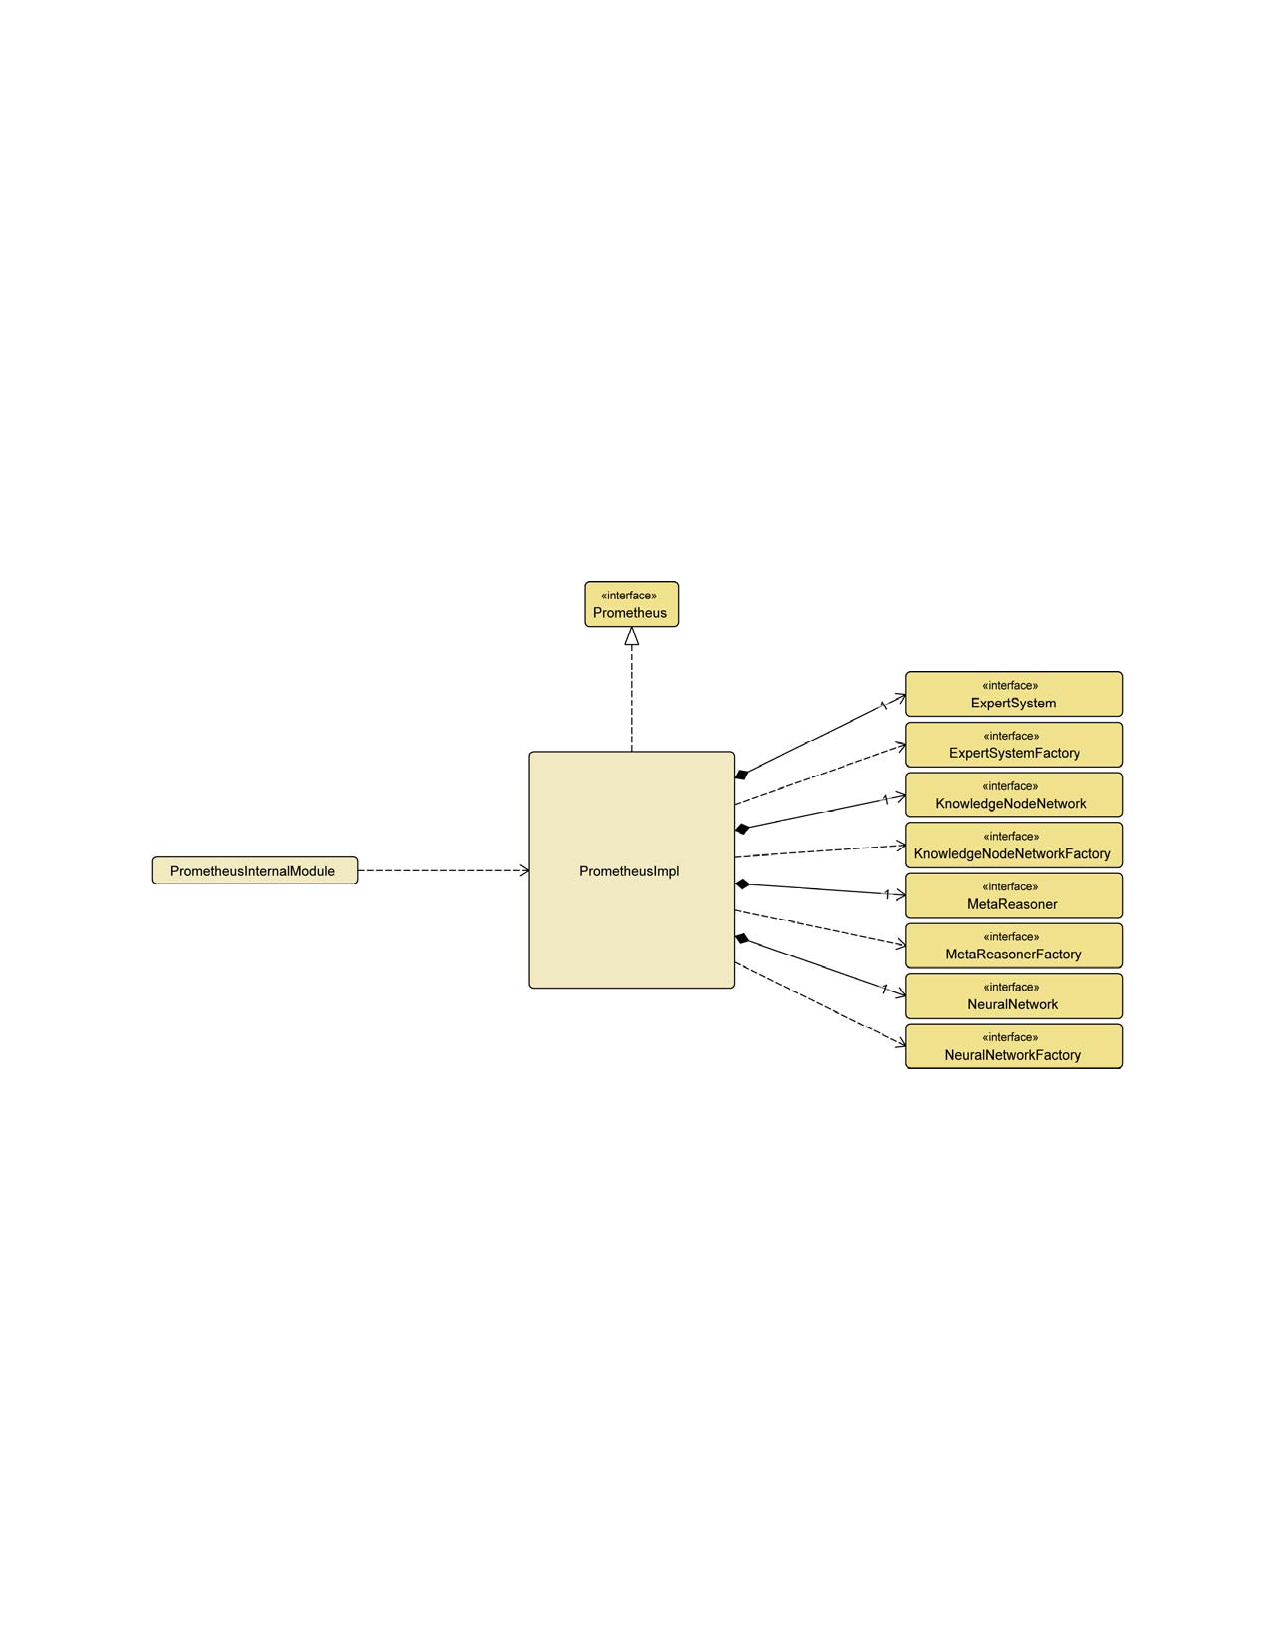
\includegraphics[width=\textwidth]{figures/prometheus_uml.pdf}
%				\caption
%				{Prometheus package.}
%			\end{subfigure}
%			~
			\begin{subfigure}[!htb]{0.4\columnwidth}
				\centering
				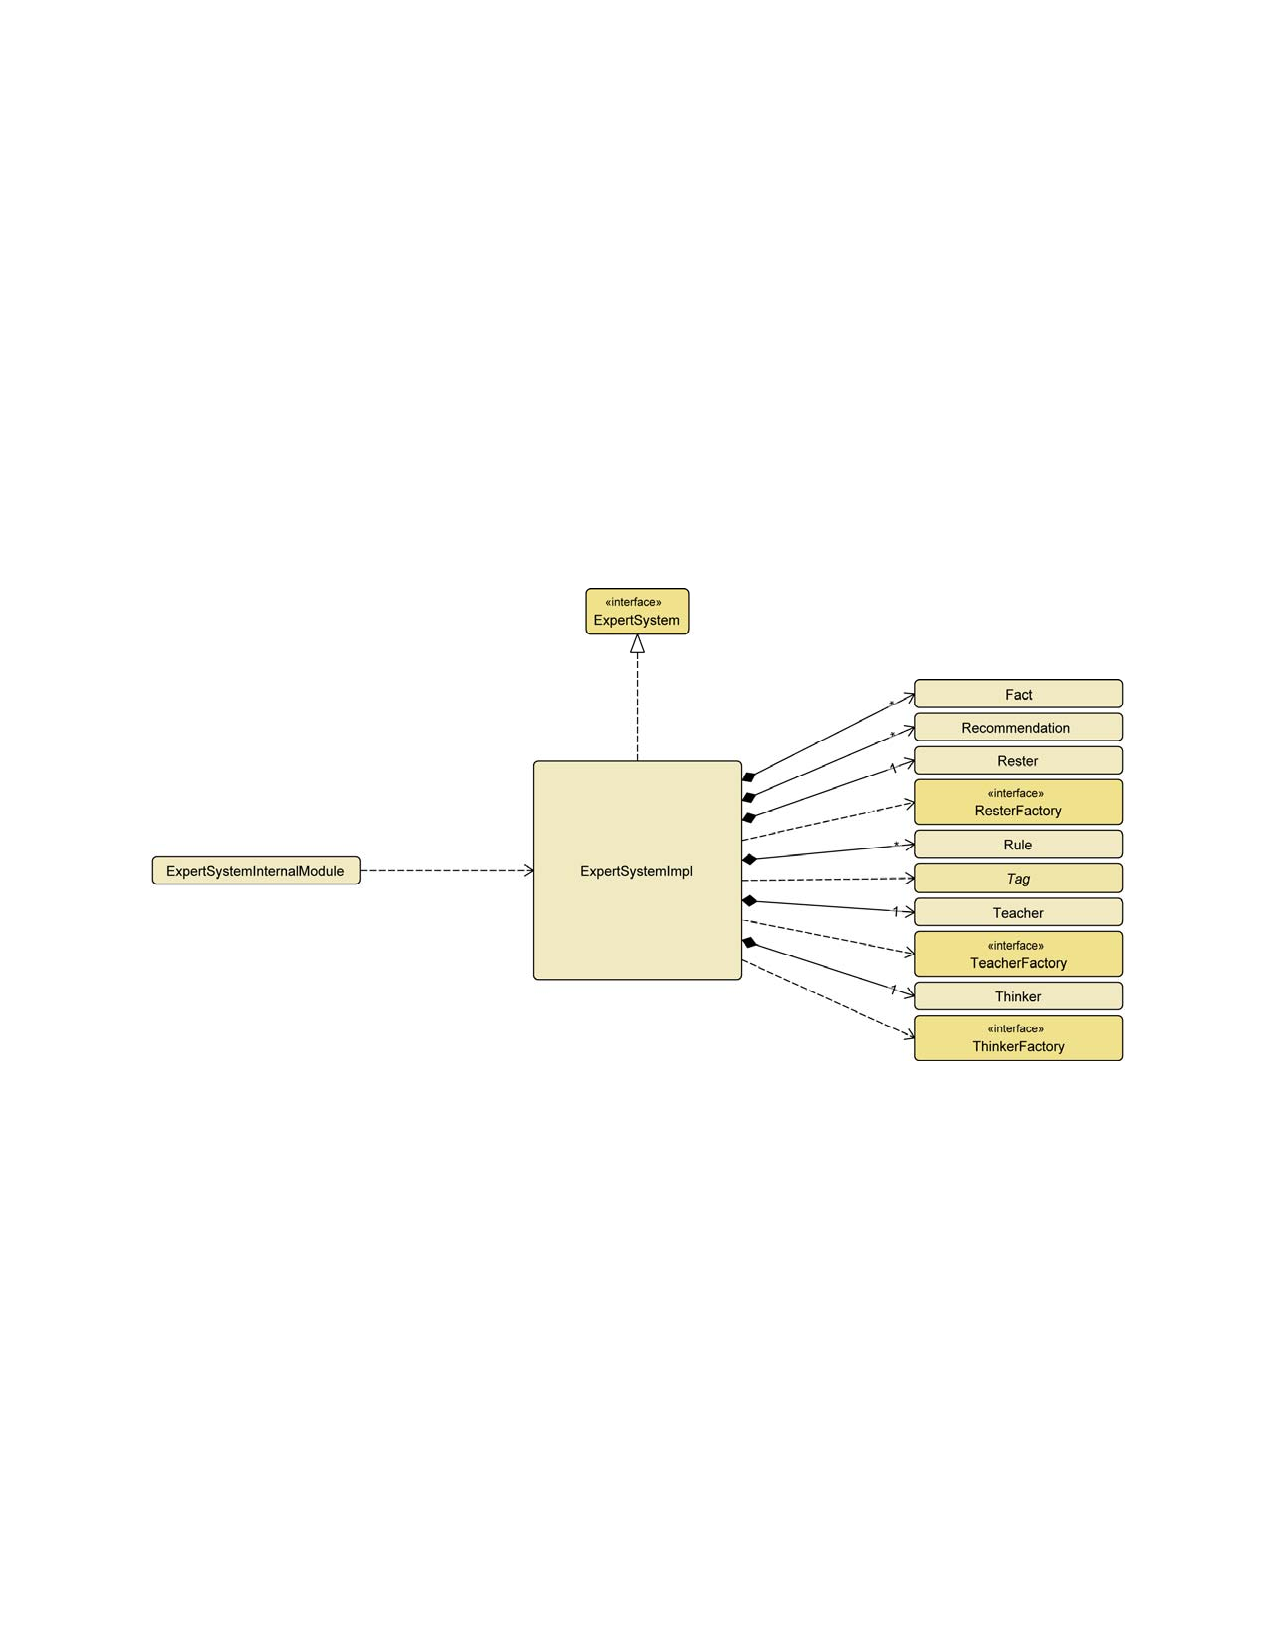
\includegraphics[width=\columnwidth]{figures/es_uml.pdf}
				\caption
				{ES package.}
			\end{subfigure}
			~
			\begin{subfigure}[!htb]{0.4\columnwidth}
				\centering
				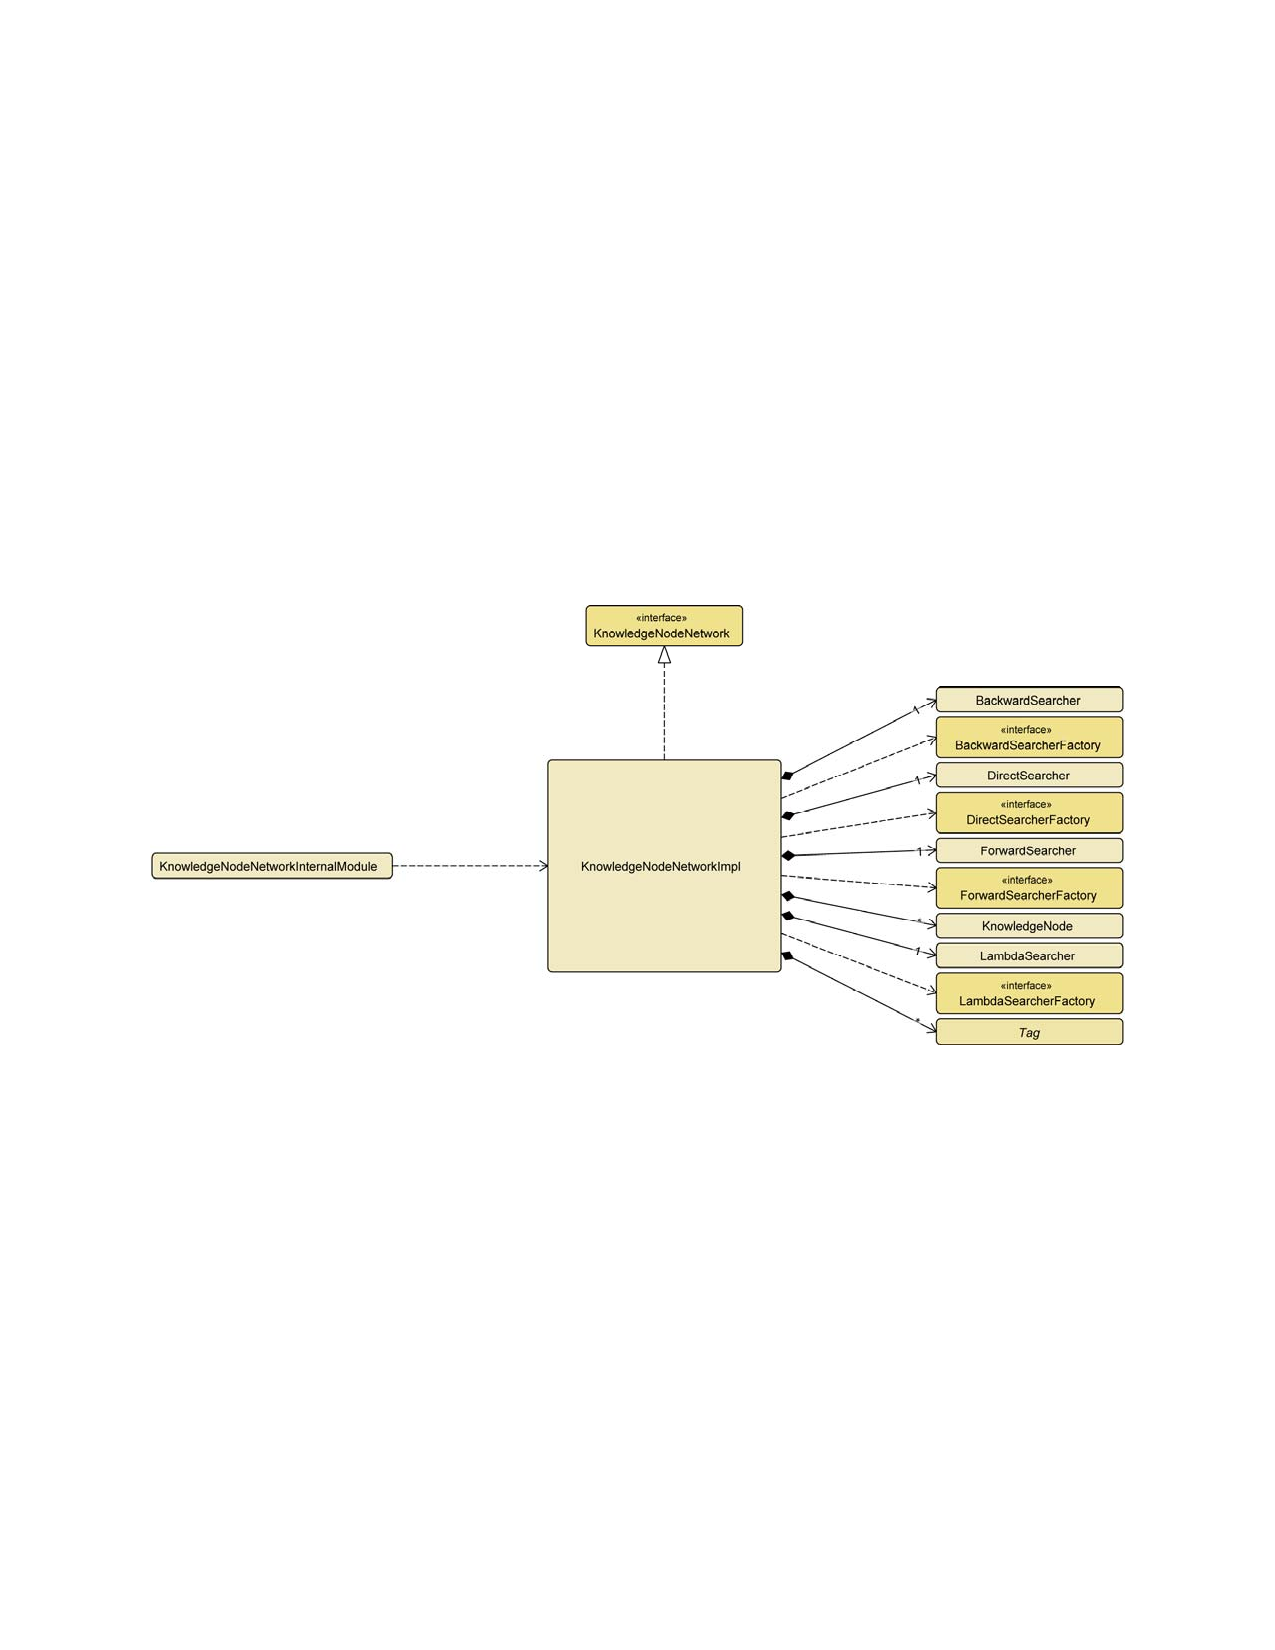
\includegraphics[width=\columnwidth]{figures/knn_uml.pdf}
				\caption
				{KNN package.}
			\end{subfigure}
			\caption{UML diagrams for the major modules.}
		\end{figure}
	
	
		\begin{figure}[!htb]
			\centering
			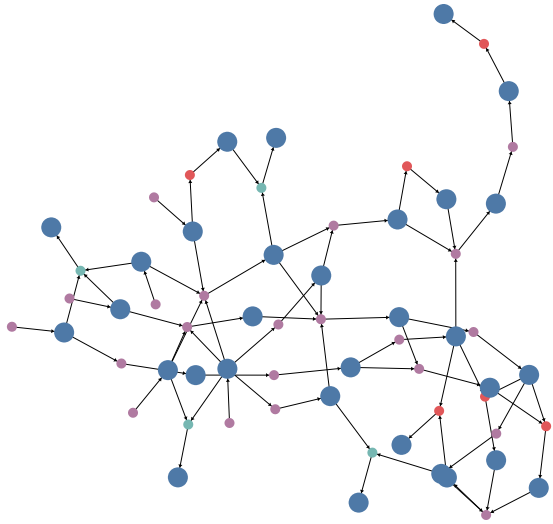
\includegraphics[width=.3\columnwidth]{figures/knn_graph.png}
			\caption{Visualization of the KNN. Small nodes are Tags, big nodes are Knowledge Nodes (KNs). Red nodes represent active Tags or fired KNs. For non-active Tags, Facts are purple, Rules are blue and Recommendations are orange.}
		\end{figure}
	
		\begin{figure}[!htb]
			\centering
			\begin{subfigure}[!htb]{0.18\columnwidth}
				\centering
				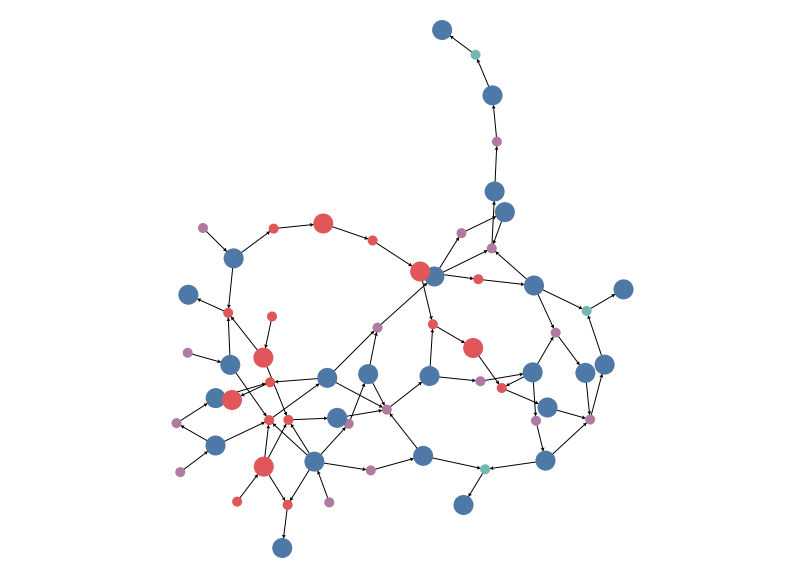
\includegraphics[width=\columnwidth]{figures/knn_forward_think_1.png}
				\caption{Ply 1.}
			\end{subfigure}
			~
			\begin{subfigure}[!htb]{0.18\columnwidth}
				\centering
				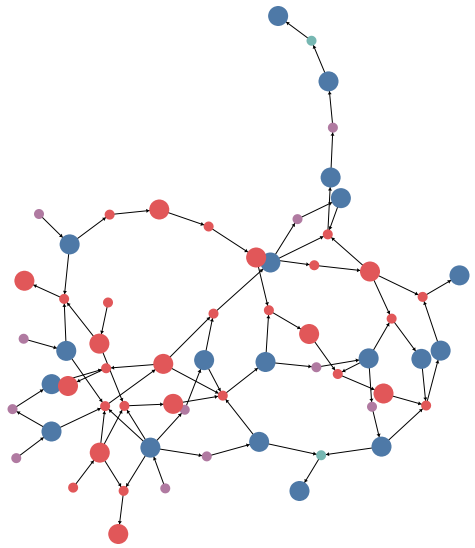
\includegraphics[width=\columnwidth]{figures/knn_forward_think_2.png}
				\caption{Ply 2.}
			\end{subfigure}
			~
			\begin{subfigure}[!htb]{0.18\columnwidth}
				\centering
				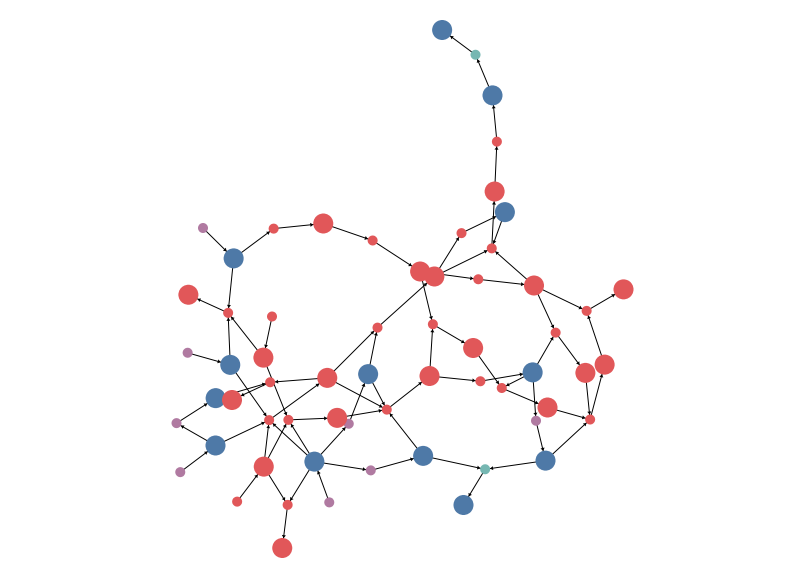
\includegraphics[width=\columnwidth]{figures/knn_forward_think_3.png}
				\caption{Ply 3.}
			\end{subfigure}
			~
			\begin{subfigure}[!htb]{0.18\columnwidth}
				\centering
				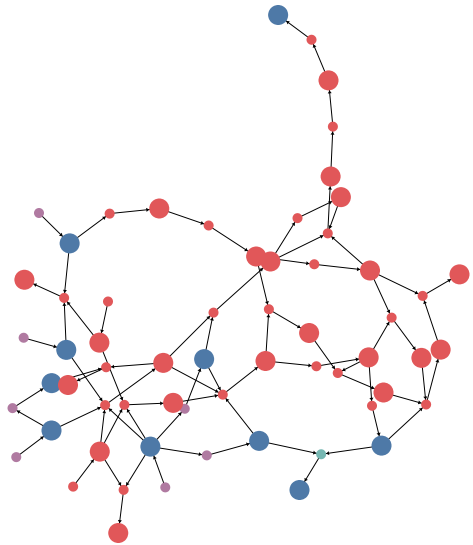
\includegraphics[width=\columnwidth]{figures/knn_forward_think_4.png}
				\caption{Ply 4.}
			\end{subfigure}
			~
			\begin{subfigure}[!htb]{0.18\columnwidth}
				\centering
				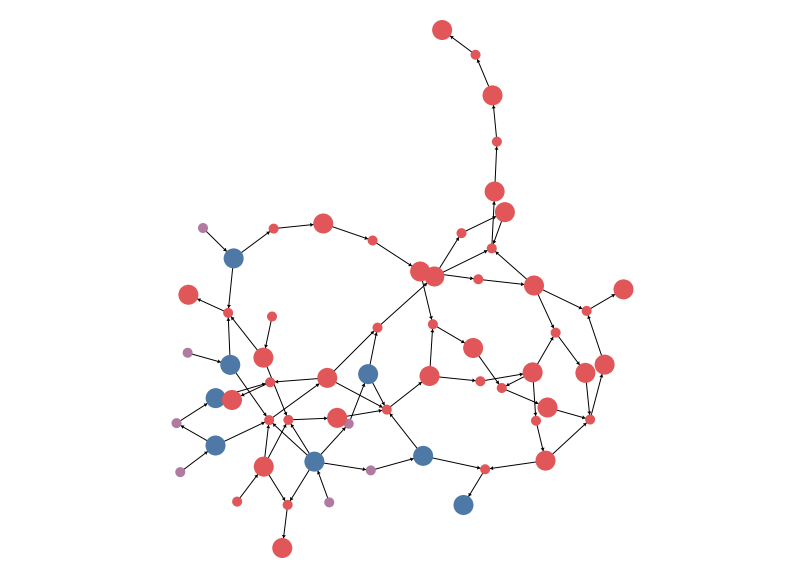
\includegraphics[width=\columnwidth]{figures/knn_forward_think_5.png}
				\caption{Ply 5.}
			\end{subfigure}
			\caption{Forward thinking visualization in the KNN.}
		\end{figure}
	
	
		\begin{figure}[!htb]
			\centering
			\begin{subfigure}[!htb]{0.18\columnwidth}
				\centering
				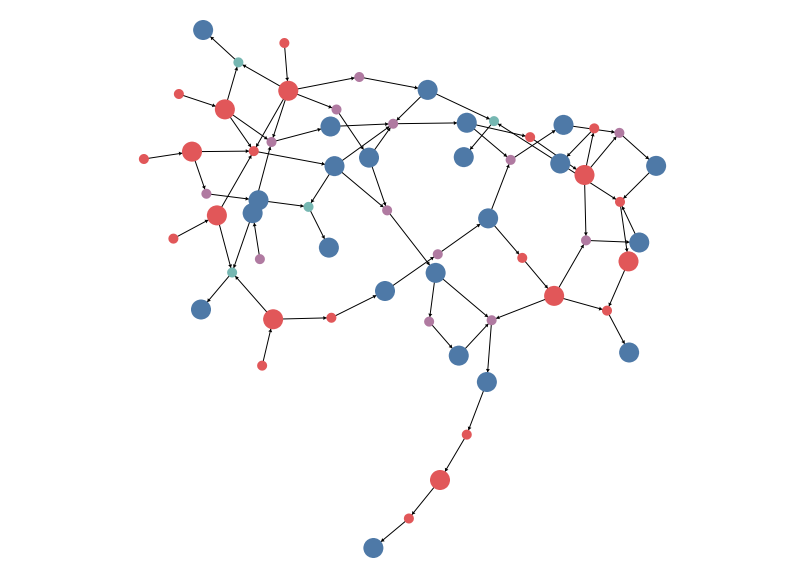
\includegraphics[width=\columnwidth]{figures/knn_backward_think_1.png}
				\caption{Ply 1.}
			\end{subfigure}
			~
			\begin{subfigure}[!htb]{0.18\columnwidth}
				\centering
				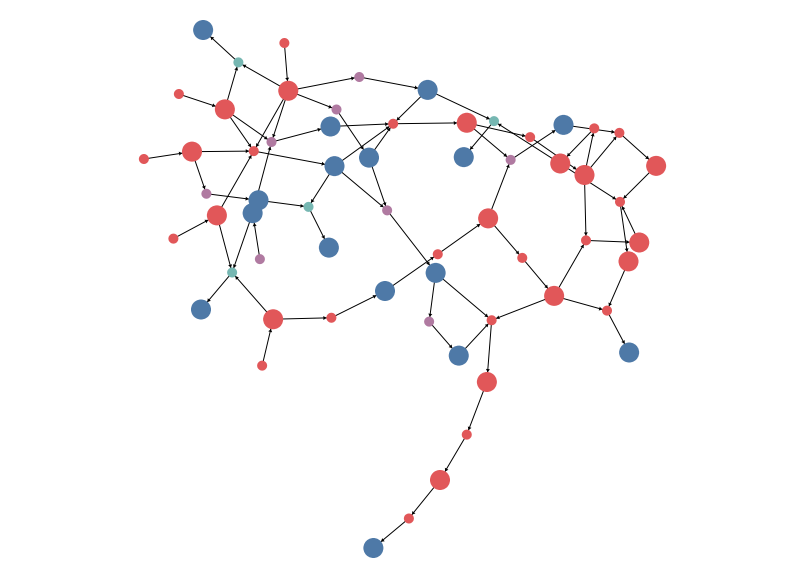
\includegraphics[width=\columnwidth]{figures/knn_backward_think_2.png}
				\caption{Ply 2.}
			\end{subfigure}
			~
			\begin{subfigure}[!htb]{0.18\columnwidth}
				\centering
				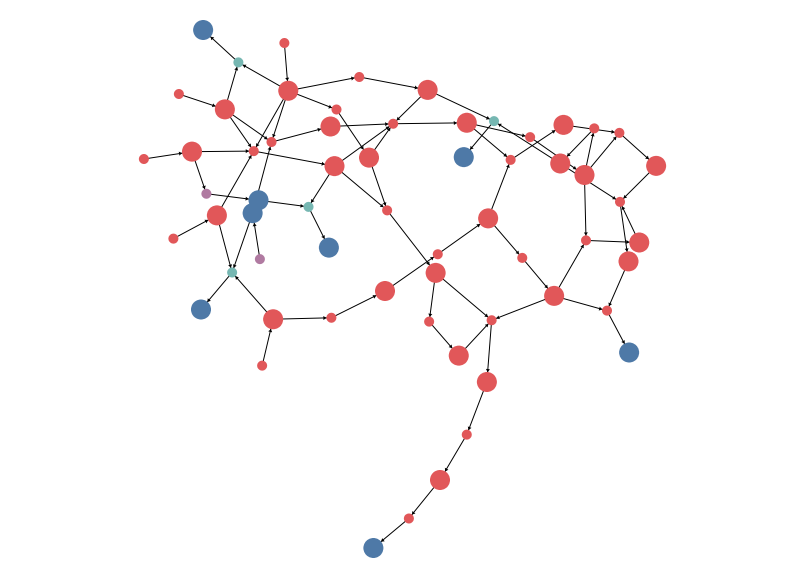
\includegraphics[width=\columnwidth]{figures/knn_backward_think_3.png}
				\caption{Ply 3.}
			\end{subfigure}
			~
			\begin{subfigure}[!htb]{0.18\columnwidth}
				\centering
				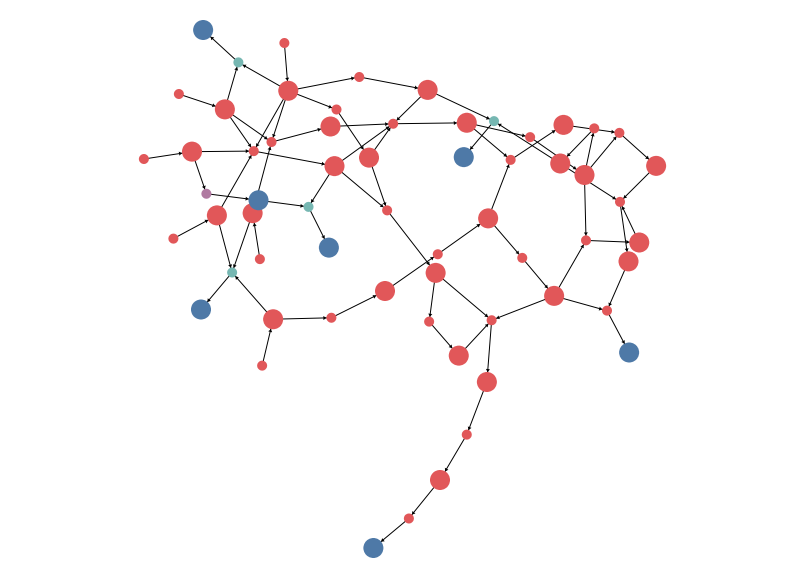
\includegraphics[width=\columnwidth]{figures/knn_backward_think_4.png}
				\caption{Ply 4.}
			\end{subfigure}
			\caption{Backward thinking visualization in the KNN.}
		\end{figure}
	
		\end{block}
	\end{column}
	\begin{column}{.3\textwidth}
		\begin{block}{Results \& Tests}
			\begin{itemize}
				\item Unit tests
				\item Integration tests
				\item TestNG and TravisCI
			\end{itemize}
		
			\begin{figure}[!htb]
				\centering
				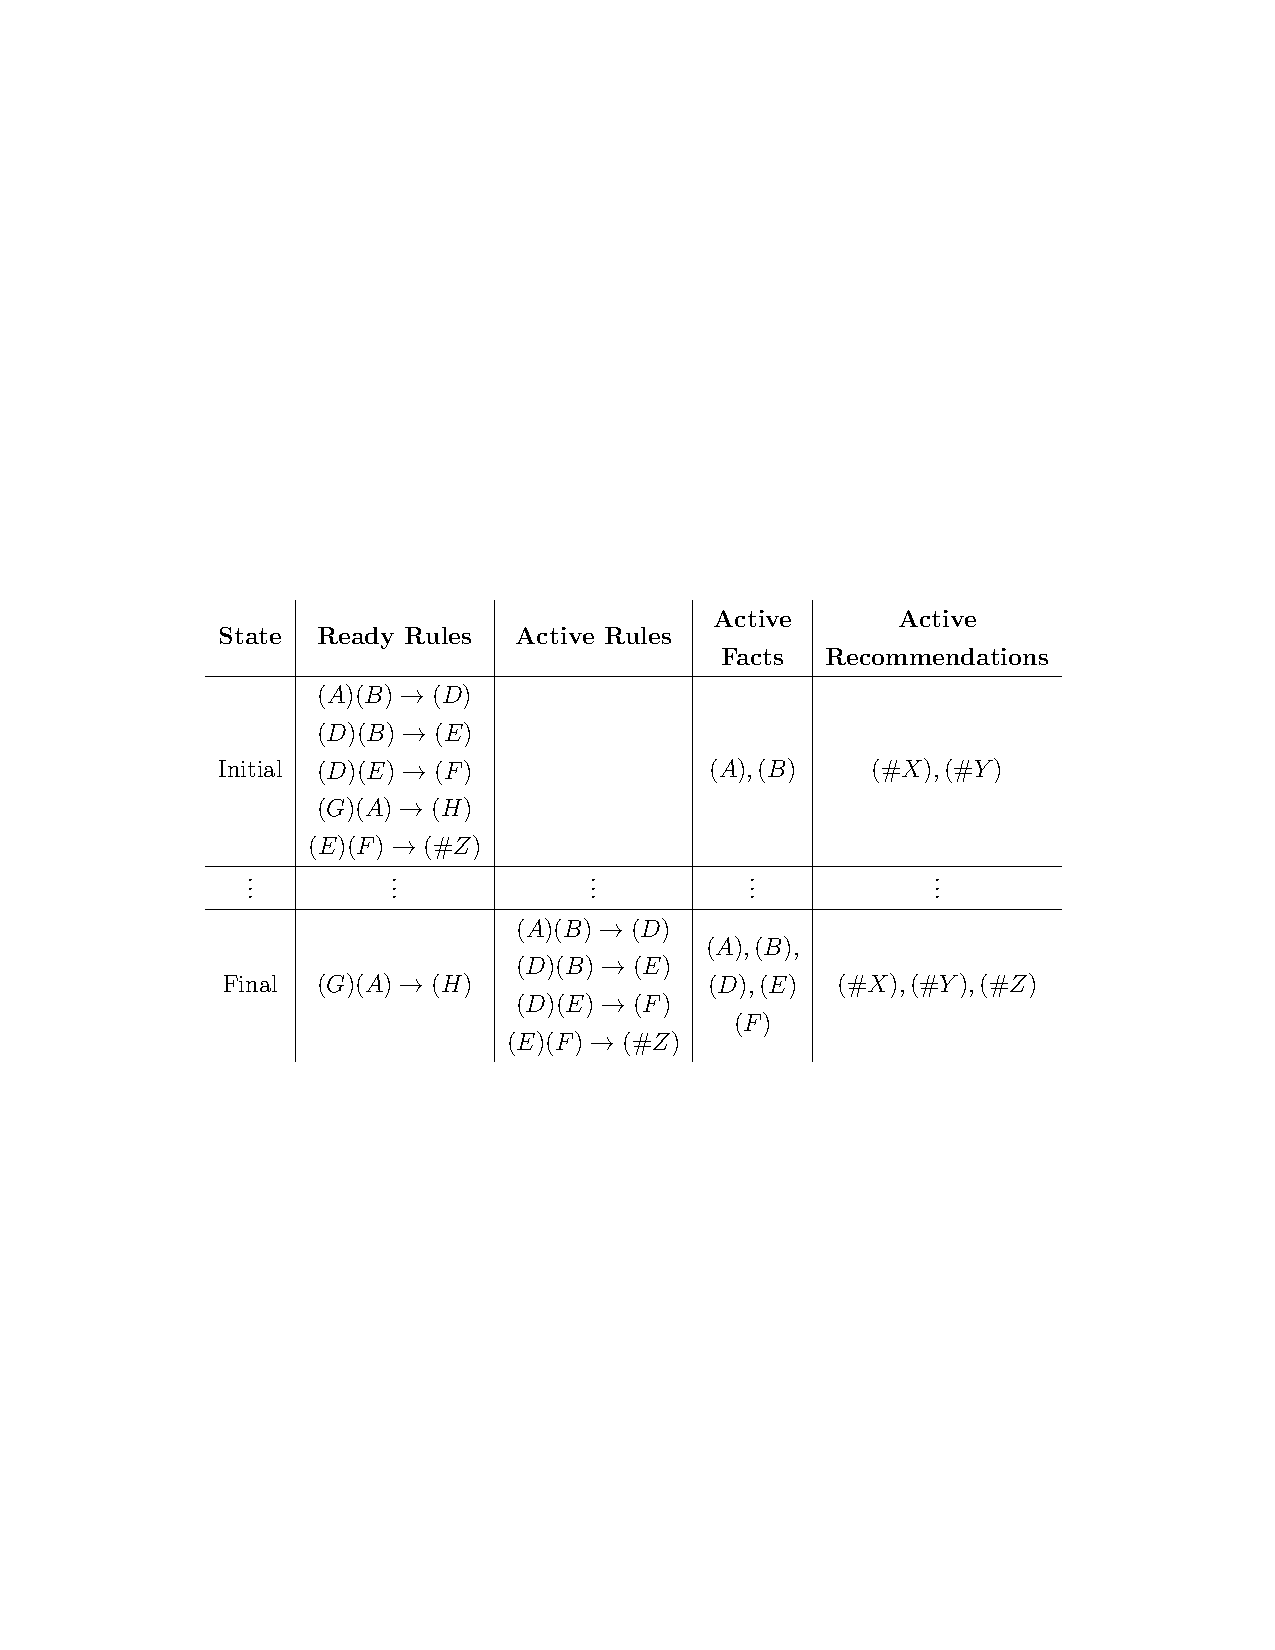
\includegraphics[width=\textwidth]{figures/testES.pdf}
				\caption
				{Simple ES test setup.}
			\end{figure}
		
			\begin{figure}[!htb]
				\centering
				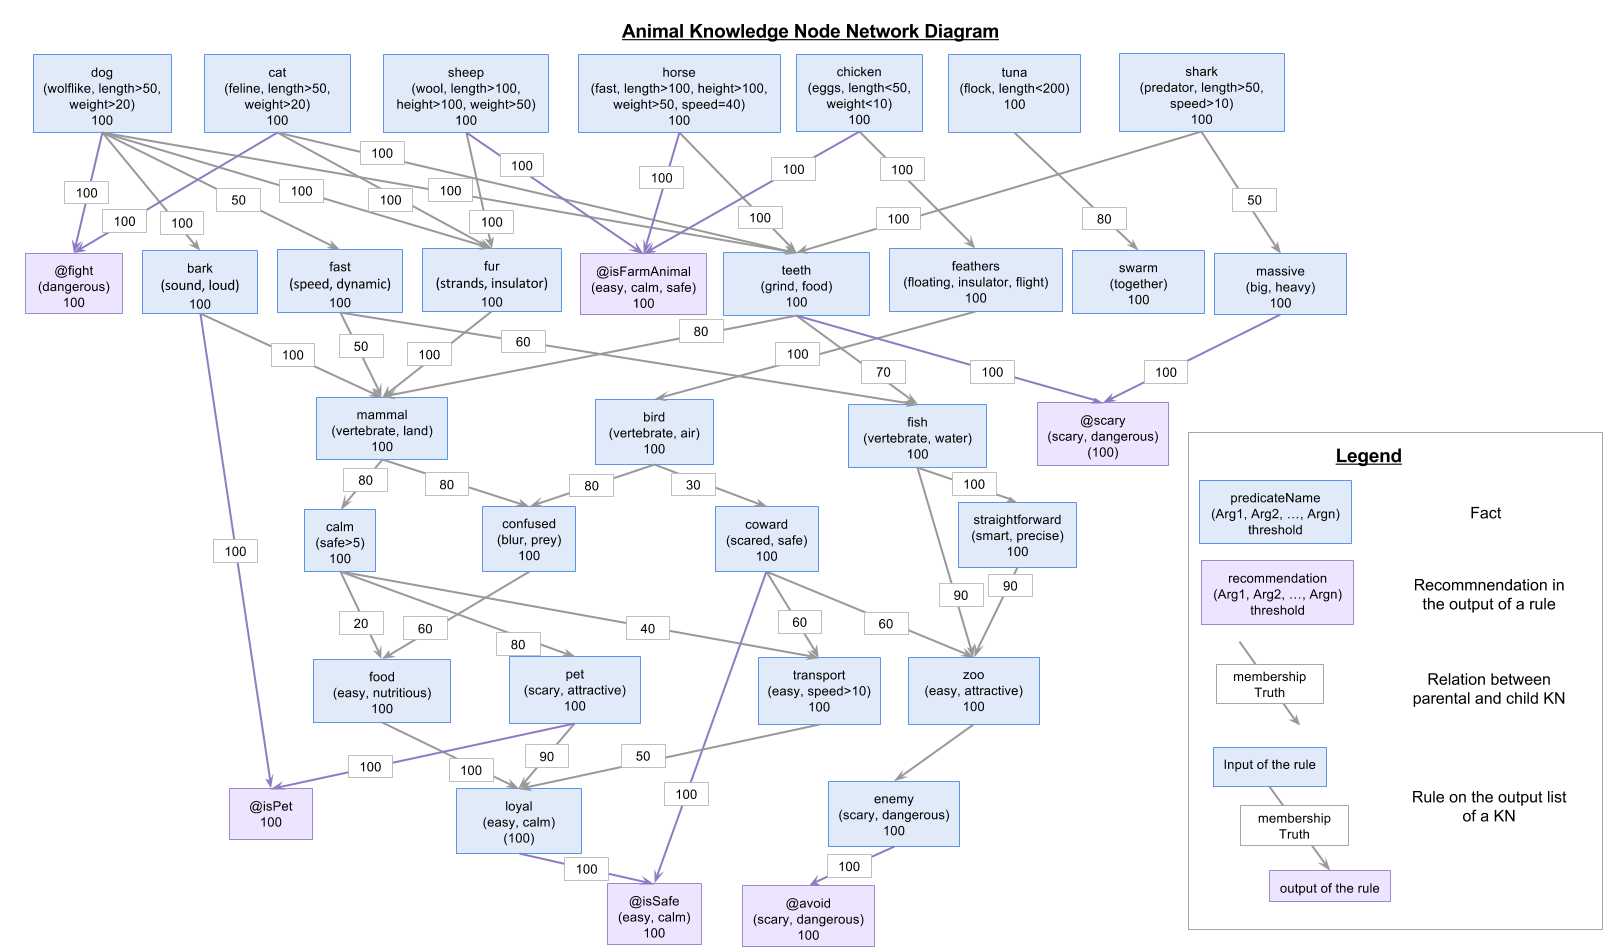
\includegraphics[width=\textwidth]{figures/animal_knn.png}
				\caption
				{Elaborate test KNN network.}
			\end{figure}
		
			\begin{figure}[!htb]
				\centering
				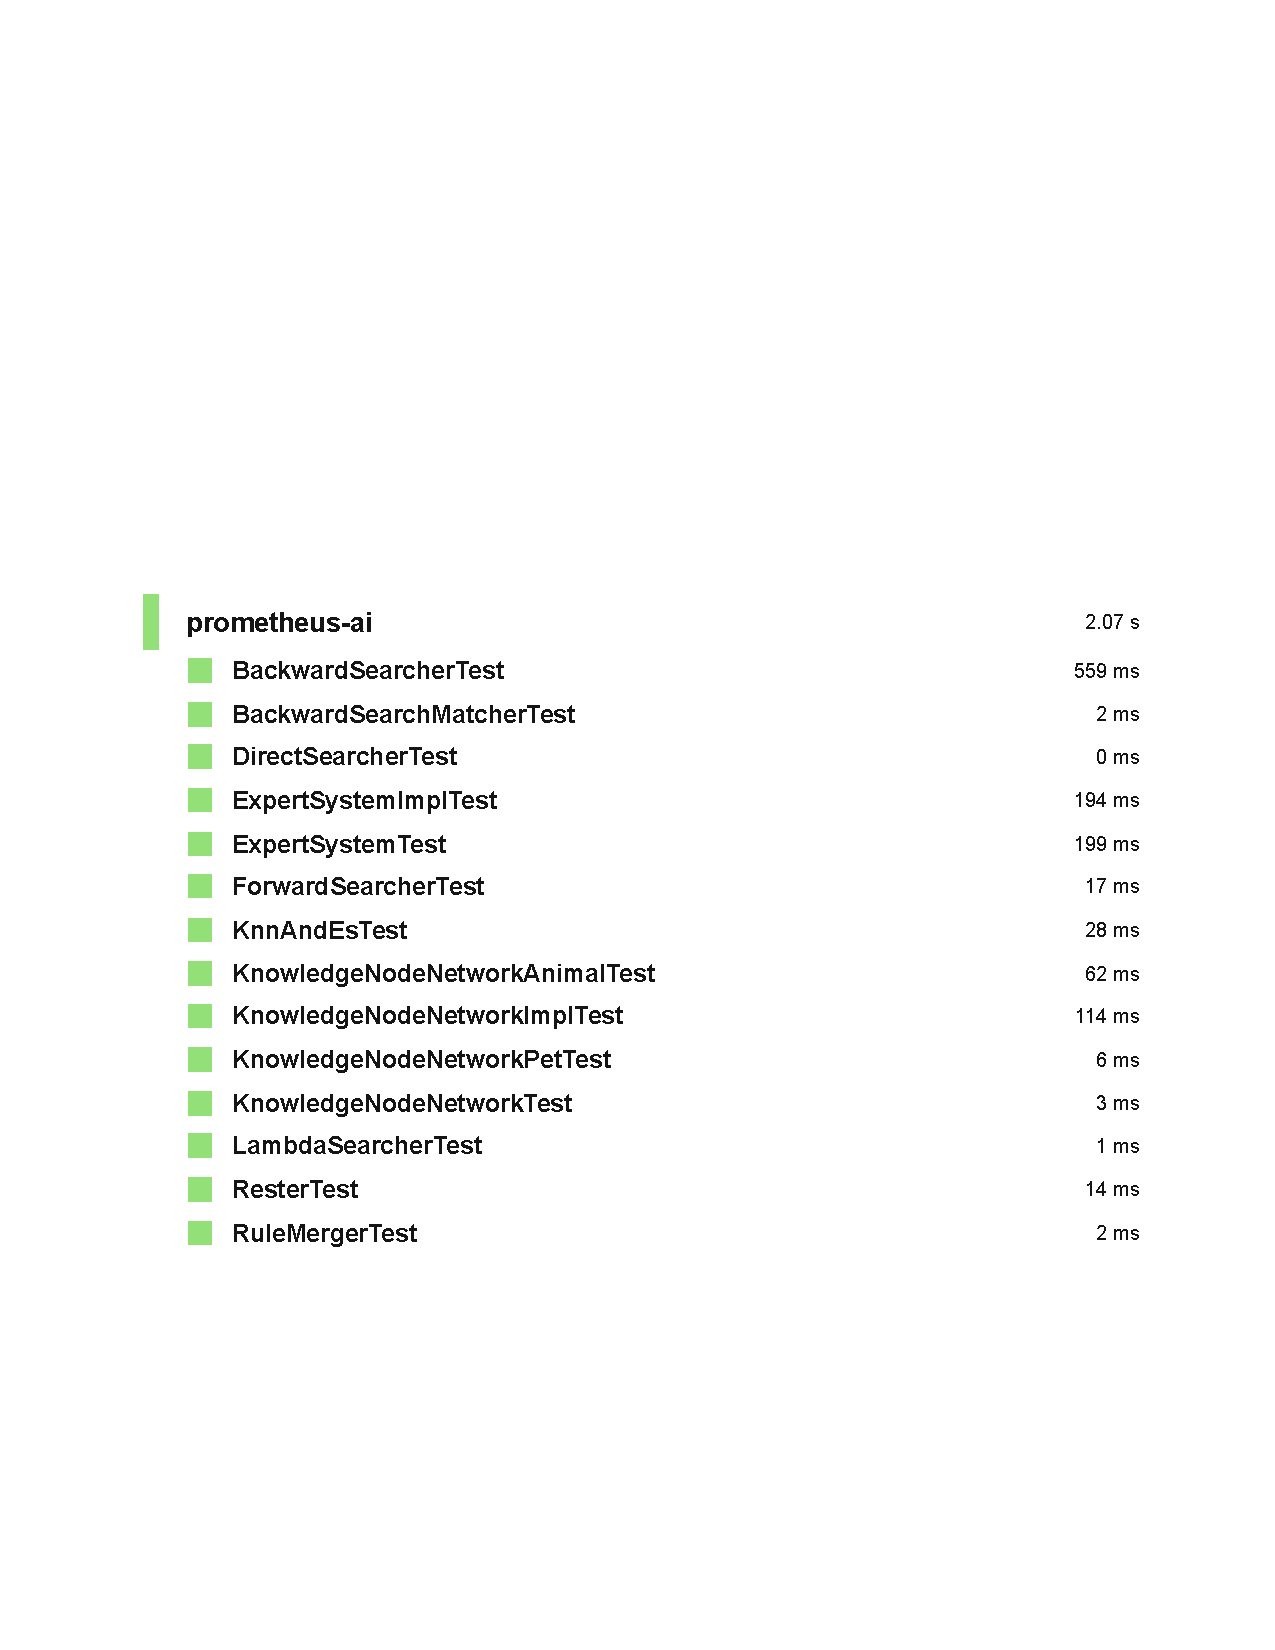
\includegraphics[width=0.5\columnwidth]{figures/test_results.pdf}
				\caption
				{Test results for various modules.}
			\end{figure}
		\end{block}
		\begin{block}{Conclusion}
		\end{block}
	\end{column}
\end{columns}
\end{document}